\documentclass[12pt]{article}
 
\usepackage[margin=.75in]{geometry} 
\usepackage{amsmath,amsthm,amssymb}
\usepackage{bm}
\usepackage{enumitem}
\setenumerate{listparindent=\parindent}

\usepackage[english]{babel}
\usepackage[utf8]{inputenc}
\usepackage{amsmath,amssymb, amsthm}
\usepackage{graphicx}
\usepackage{amssymb}
\usepackage{verbatim}
\usepackage{gensymb}
\usepackage{bm}

\usepackage{tikz}
\usepackage{tkz-berge}
%\usepackage{graphics,graphicx}
%\usepackage{pstricks,pst-node,pst-tree}
\usepackage[colorinlistoftodos]{todonotes}
\usetikzlibrary{arrows,shapes,positioning}
%\usetikzlibrary{positioning,arrows}
 
 
\newcommand{\N}{\mathbb{N}}
\newcommand{\Z}{\mathbb{Z}}
\newcommand{\p}{\mathcal{P}_2(T)}
\newcommand{\Aut}{\textnormal{Aut}(P)}

 
\begin{document}
 
% --------------------------------------------------------------
%                         Start here
% --------------------------------------------------------------


\title{Math 172 - HW 4}
\author{Michael Knopf}
 
\maketitle

%%%%%%%%%%%%%%%%%%%%     1     %%%%%%%%%%%%%%%%%%%%%%%%

\begin{enumerate}[leftmargin=0cm,itemindent=.5cm,labelwidth=\itemindent,labelsep=0cm,align=left]

\item Show that a finite \emph{regular} (meaning each vertex has the same positive degree) bipartite graph has a perfect matching.

\begin{proof}

\ Let $G = A \cup B$ be a disjoint union satisfying the bipartite condition.  Since every vertex has the same degree $d > 0$, we have $d|A| = |E(G)| = d|B|$.  So $|A| = |B|$.  Therefore, if $G$ has a complete matching from $A$ to $B$, then that matching must be perfect: the complete matching will induce an injection $A \rightarrow B$, which must be a bijection since $|A| = |B|$.

To show that $G$ satisfies the hypothesis of Hall's Theorem, let $S \subseteq G$.  Then there are $d|S|$ edges leaving $S$ and entering $\Gamma(S)$, since all vertices joined with vertices in $S$ are represented in $\Gamma(S)$.  There are $d|\Gamma(S)|$ total edges entering $\Gamma(S)$.  Therefore, $d|S| \leq d|\Gamma(S)|$.  So $|S| \leq |\Gamma(S)|$, thus Hall's Theorem is satisfied.  By the argument in the previous paragraph, a perfect matching exists.

\end{proof}

\item Find the chromatic polynomial $\raisebox{3pt}{$\chi$}_G$ for the $n$-cycle $C_n$ and the $n$-wheel $W_n$.  The graph $W_n$ is defined as the graph obtained from $C_n$ by adding a new vertex $v$ and joining it to all vertices of $C_n$.

\begin{figure}[h!]
\begin{center}
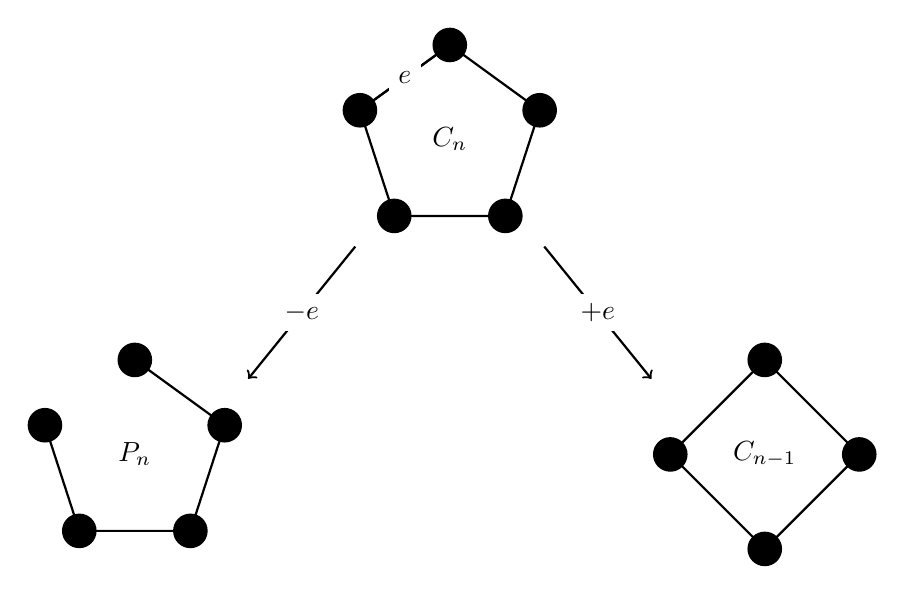
\begin{tikzpicture}[rotate = 90, scale = .8]
\SetVertexNoLabel
\SetVertexSimple
\grCycle[RA=1.5]{5}
\Edge[label=$e$](a0)(a1)
\node(0,0) {$C_n$};

\begin{scope}[shift = {(-5cm, 5cm)}]
\SetGraphUnit{1.5}
\Vertices{circle}{A,B,C,D,E}
\Edges(B,C,D,E,A)
\node(0,0) {$P_n$};
\end{scope}

\begin{scope}[shift = {(-5cm, -5cm)}]
\grCycle[RA=1.5]{4}
\node(0,0) {$C_{n-1}$};
\end{scope}

\coordinate (A) at (-1.7,1.5);
\coordinate (B) at (-3.8,3.2);
\draw[->, thick] (A) -- (B) node[midway,fill=white] {$-e$};

\coordinate (A) at (-1.7,-1.5);
\coordinate (B) at (-3.8,-3.2);
\draw[->, thick] (A) -- (B) node[midway,fill=white] {$+e$};

\end{tikzpicture}
\end{center}
\end{figure}

\begin{proof}
\ Denote by $G-e$ the graph obtained by deleting the edge $e$ from $G$, and by $G+e$ the graph obtained by contracting the edge $e$ in $G$.  Also, whenever $\raisebox{3pt}{$\chi$}_G$ is written, assume the number of colors being used is $k$.

Contracting an edge in $C_n$ results in $C_{n-1}$.  Deleting an edge from $C_n$ results in a path graph on $n$ vertices.  The number of ways to color $P_n$ with $k$ colors is $k(k-1)^{n-1}$, since the first vertex can be colored any color, and each consecutive vertex can be colored any color except for the color of the vertex before it.  Therefore, $$\raisebox{3pt}{$\chi$}_{C_n} = k(k-1)^{n-1} - \raisebox{3pt}{$\chi$}_{C_{n-1}}.$$

The homogeneous solution to this recurrence is $c(-1)^n$ for some constant $c$.  It is easy to see by inspection that a particular solution is given by $\raisebox{3pt}{$\chi$}_{C_n} = (k-1)^n$.  So the general solution is of the form $\raisebox{3pt}{$\chi$}_{C_n} = (k-1)^n + c(-1)^n$.  Since $C_3 = K_3$, we know that $\raisebox{3pt}{$\chi$}_{C_3} = \raisebox{3pt}{$\chi$}_{K_3} = k(k-1)(k-2)$.  Thus,
\begin{align*}
k(k-1)(k-2) &= (k-1)^3 + c(-1)^3 \\
k^3 - 3k^2 + 2k &= k^3 - 3k^2 + 3k - 1 - c \\
c &= k - 1
\end{align*}
So the general solution is $$\raisebox{3pt}{$\chi$}_{C_n} = (k-1)^n + (k-1)(-1)^n.$$

To color $W_n$, first choose a color for the center vertex.  Next, color the outside vertices (which form a subgraph isomorphic to $C_n$) with the remaining $k-1$ colors.  Therefore,
$$
\raisebox{3pt}{$\chi$}_{W_n}(k) = k \cdot \raisebox{3pt}{$\chi$}_{C_n}(k-1) = k(k-1)^{n-1} + k(k-1)(-1)^{n-1}
$$

\end{proof}

\item Find the number of ways to place 3 rooks on the $8 \times 8$ chessboard such that no two rooks attack each other.

\begin{proof}

\ First, choose the 3 ranks to place the rooks in: $\binom{8}{3}$.  Next, choose a file for each of those ranks: $(8)_3$.  So this can be done in $\binom{8}{3} (8)_3$ ways.  Alternatively, we have $8^2$ choices for the first rook, $7^2$ choices for the second, and $6^2$ for the third.  However, we have overcounted because permutations of the rooks have been counted as unique.  So the answer is $\dfrac{8^2 7^2 6^2}{3!}$.

\end{proof}

\item (optional) Tell me why I shouldn't submit my 4-color theorem proof to the \emph{Annals of Mathematics}.

\item Let $G$ be a simple graph with 10 vertices and 26 edges.  Show that $G$ has at least 5 triangles.

I have tried tirelessly, and in vain, to solve this problem without help, but could not come up with anything.  In a post on stackexchange, someone stated the following theorem (without proof):

\noindent \emph{``Any graph on $2n+\delta$ nodes(where $\delta$ is 0 or 1) with exactly $n(n+\delta)+1$ edges has at least $n$ triangles."}

The only statement they made about its proof was: ``If I recollect correctly, this can be proved by induction on $n$, by showing that there is a vertex of degree $\leq n$ and then deleting it to try and apply the induction hypothesis."  The given problem is the special case where $n = 5$ and $\delta = 0$.  However, the cases where $\delta = 1$ are necessary to prove as well, since they are used in the inductive step.  I will prove this more general theorem.

\begin{proof}

\ Induct on $n$.  When $n=0$ and $\delta = 0$, $G$ is a graph with $0$ vertices and 1 edge; when $n = 0$ and $\delta = 1$, $G$ is a graph with $1$ vertex and 1 edge.  The set of graphs of satisfying these conditions is empty, thus the proposition is vacuously true for $n = 0$ and $n = 1$.

When $n = 1$ and $\delta = 0$, $G$ is a graph with 2 vertices and 3 edges, so again the statement holds vacuously.  When $n = 1$ and $\delta = 1$, $G$ is a graph with 3 vertices and 3 edges, which is a triangle, thus $G$ contains $n=1$ triangle.

Now, suppose the proposition is true for $n-1$, and suppose $G$ is a graph with $2n$ vertices and $n^2 + 1$ edges (here we are showing the case where $\delta = 0$).  The average degree of the graph is
$$
\frac{2(n^2 + 1)}{2n} = n + \frac1n < n+1
$$
since $n > 1$.  Thus there exists a vertex with degree less than or equal to $n$.

First, suppose there exists some vertex $x$ with degree $k$ strictly less than $n$.  Now, consider the graph $H$ formed by removing the $x$ (and all edges incident with it) from $G$.  $H$ now has $2n-1 = 2(n-1) + 1$ vertices and $$n^2 - k + 1 > n^2 - n + 1 = n(n-1) + 1 = (n-1)((n-1) + 1) + 1$$ edges.  Remove $n-k$ edges from $H$ to retrieve a subgraph with exactly $(n-1)((n-1) + 1) + 1$ edges.  This subgraph satisfies the hypothesis of the proposition for $n-1$ when $\delta = 1$, thus it contains $n-1$ triangles.  Since a subgraph of $H$ contains $n-1$ triangles, $H$ contains them as well.

Let $\{a,b,c\}$ be one of these triangles.  Now, consider the graph $K$ formed by removing the edge $(a,b)$ from $H$.  Since $H$ had \emph{strictly} more than the amount of edges necessary for the proposition for $n-1$, $K$ has \emph{at least} enough edges to satisfy the proposition.  Thus $K$ has $n-1$ triangles.  However, $K$ does not contain the triangle $\{a,b,c\}$.  Therefore, $H$ must have had $n$ triangles all along.  So $G$ contains $n$ triangles.

Now, suppose that $G$ contains no vertices with degree strictly less than $n$.  Then it contains a vertex $x$ with degree exactly $n$.  Again, let $H$ be the subgraph obtained by removing $x$ and all incident edges from $G$.  $H$ has $2n-1$ vertices and $n^2 - n +1$ edges, thus it again satisfies the hypothesis of the proposition for $n-1$.  So $H$ contains $n-1$ triangles.

Let $\{a,b,c\}$ be one of these triangles, and assume that none of $a$, $b$, or $c$ have degree $n$.  Then these 3 vertices in $H$ have degree at least $n+1$.  So the total degree of $H$ is greater than or equal to $3(n+1) + (2n-4)n = 2n^2 - n + 3$.  However, we know that the total degree of $H$ is $2n^2 -2n + 2$.  So this implies
\begin{align*}
2n^2 - n + 3 &\leq 2n^2 - 2n + 2 \\
n &\leq -1
\end{align*}
which is a contradiction.  So at least one of $a$, $b$, and $c$ has degree $n$.  Assume WLOG that it is $a$.

Let $K$ be the graph formed by removing $a$ and all incident edges from $G$.  Then $a$ is no different than $x$ was in our construction of $H$, thus $K$ also has $n-1$ triangles.  However, $K$ does not contain the triangle $\{a,b,c\}$.  Therefore, $G$ must have $n$ triangles.  This completes the case where $\delta = 0$.

Now, assume $\delta = 1$.  Then $G$ has $2n+1$ vertices and $n(n+1)+1 = n^2 + n + 1$ edges.  So the average degree of $G$ is
$$
\frac{2(n^2 + n + 1)}{2n+1} = \frac{2n^2 + n + n + 2}{2n+1} = n + \frac{2+n}{2n+1} < n
$$
because $n > 1$ (so $2+n < 2n+1$).  Therefore, $G$ contains a vertex $x$ of degree $n$.  The subgraph $H$ formed by removing $x$ and all incident edges has $2n$ vertices and $n^2 + 1$ edges.  This is simply the case where $\delta = 0$, which we have just proved.  So $H$ contains $n$ triangles, thus $G$ contains $n$ triangles.
\end{proof}

\item What is $$\sum\limits_{k=0}^n k \binom{n}{k}?$$

\begin{proof}

\ The summand counts the number of ways to pick $k$ peasants from a country of $n$ people and knight them lords, then choose 1 of these lords to be king of all the land.  Summing these all up counts the number of ways to pick any number of peasants from the land and knight them lords, then choose 1 of them to be king.

This can be done without the summation.  Simply pick the king \emph{first}, which can be done in $n$ ways, then choose some other peasants to serve as lords below him, which can be done in $2^{n-1}$ ways, since the king cannot be chosen as a lord.  Thus, this summation equals $n 2^{n-1}$.

\end{proof}

\item How much time did you spend on this problem set?  What comments do you have on the problems?

I'm not sure how much time I spent on this, but most of it was spent on \# 5.  What made it so difficult was that it was stated as a special case of a more general proposition for which the proof is much easier to think of than the case analysis I assume would have been necessary to solve the given scenario.  If this really was the way the problem was intended to be solved, I would have rather it been stated in the more general form.  Possibly I haven't invested enough of my free time into studying graphs with $2n + \delta$ vertices and $n(n+\delta) + 1$ edges to immediately think of $2 \cdot 5$ and $5^2 + 1$ whenever I see the numbers $10$ and $26$ together.  I was about ready to try to make a connection between the base of our number system, the number of letters in the alphabet, and graphs with at least 5 triangles, but surprisingly this turned out to be a dead end.

Once I decided to prove the more general statement for \# 5, I still had trouble because I was trying to ignore the case where $\delta = 1$.  However, this creates a missing link in the induction.

\# 1 was difficult at first because I thought I could solve it more easily without using Hall's Theorem, but I think I was wrong about that.  I thought I could show it easily by induction, by deleting edges to produce a smaller regular bipartite graph, but it ended up being more complicated than it was worth.  I think it's true, though, that any finite regular bipartite graph where each vertex has degree $n$ should have a regular bipartite graph where each vertex has degree $n-1$.

I'm glad that 2 was on here.  It was really useful to get some practice with the chromatic polynomial.

\end{enumerate}
\end{document}



















